\documentclass{article}
\usepackage{amsmath}
\usepackage{amsfonts}
\usepackage{geometry}
\usepackage{graphicx}
\usepackage{hyperref}
\usepackage{cleveref}
\usepackage{natbib}
\usepackage{authblk}
\geometry{margin=1in}

\title{Maxwell--Boltzmann Dynamics in Cognitive Performance: A Mathematical Framework for Skill-Dependent Asymmetric Load Modeling}
\author{Wes Bailey}
\affil{Par Not Far, Inc.}
\date{Version 1.0, August 2025}

\begin{document}

\maketitle

\begin{abstract}

We present a mathematical framework for modeling cognitive performance as a function of cognitive load, inspired by
resource distribution dynamics that naturally produce the rapid rise and gradual decline seen in real-world skill
execution. By moving beyond traditional symmetric models, our approach captures the asymmetric, skill-dependent patterns
of human performance and reveals that, as expertise increases, the underlying mathematics representing cognitive load
become fundamentally simpler—a reflection of the cognitive streamlining achieved through practice. The framework also
extends to account for dynamic changes in cognitive load over time, providing a quantitative basis for understanding and
managing performance in demanding environments such as sports, medicine, and other high-stakes domains.

\end{abstract}

\section*{Introduction}

The relationship between cognitive load and performance represents a fundamental challenge in mathematical psychology: 
how to model the asymmetric, skill-dependent dynamics of human cognitive processing under varying demand conditions. 
While traditional approaches employ symmetric functions (e.g., Gaussian) to represent the inverted-U relationship 
between arousal and performance, but empirical evidence reveals systematic asymmetric cognitive load that these models
cannot capture (see, e.g., \citep{hockey1997compensatory, baumeister1984choking, beilock2001choking}): rapid
performance gains at low load followed by gradual, capacity-constrained decline at high load, with the degree of
asymmetry varying systematically with expertise level. 

This paper develops a mathematical framework that addresses these limitations by introducing a Maxwell-Boltzmann-
inspired formulation for cognitive performance modeling. The approach is motivated by three key theoretical insights: 
(1) cognitive resources follow distribution patterns similar to energy systems in constrained environments, (2) 
expertise fundamentally alters the mathematical complexity of cognitive processing, and (3) the asymmetric nature 
of performance curves reflects working memory constraints and resource allocation efficiency.

\section*{Theoretical Motivation and Contributions}

The Maxwell-Boltzmann framework is adopted here because cognitive performance under load exhibits patterns reminiscent
of particle energy distributions in constrained systems: a rapid initial mobilization of resources followed by a slow
decay as capacity limits are approached.  This paper will introduce and infer that the rise is best modeled as a
power-law ($C^{\alpha}$) and the decay is best modeled as an exponential ($e^{-kC}$), while maintaining mathematical
tractability and being interpretible.

The primary mathematical contribution is the derivation of a closed-form solution for the effective performance envelope
$A_{eff}$, which quantifies the cognitive bandwidth available for decision-making above a performance threshold.
Analysis will show that the complexity of $A_{eff}$ systematically decreases with skill level, providing a quantitative
foundation for the hypothesis, that skill whether acquired through practice or occurring naturally, simplifies cognitive
processing.

Additionally, the framework is extended to model dynamic cognitive load evolution through a set of interdependent
equations, capturing how fatigue and pressure accumulate over time and impact performance capacity. This enables the
modeling of real-time cognitive load management in extended performance events.

Overall, this unified framework integrates established cognitive theories (such as the Yerkes-Dodson law and Cognitive
Load Theory) with novel mathematical formulations. It addresses a key gap in the literature by providing a
skill-adjustable, asymmetric performance function that is both theoretically grounded and practically applicable. The
resulting model is mathematically elegant—relying on a single equation with three interpretable parameters—making it
suitable for adaptive systems and real-time applications, and representing an advance in the mathematical modeling of
cognitive performance.  It also introduces a time dependent model that can be used to model the evolution of cognitive
load and performance for extended events.

\section*{Background and Literature Review}

\subsection*{The Yerkes-Dodson Law and Performance}

The relationship between mental stimulation and performance has roots in a 1908 experiment by Yerkes and Dodson, who
observed how varying levels of electric shock affected habit formation in mice. Their results described an inverted-U
relationship: moderate stimulation produced optimal learning, while too little or too much hindered it
\citep{yerkes1908}. Although originally applied to learning, the Yerkes-Dodson law has since been widely generalized
across psychology to describe how performance in attention and decision-heavy tasks depends on stimulation levels. Low
stimulation leads to boredom or distraction; excessive stimulation causes anxiety and reduced focus—especially in
activities demanding precise motor execution or judgment under pressure \citep{diamond2005}.

\subsection*{Cognitive Demands in Sports}

Sports performance is inherently cognitive, requiring athletes to interpret dynamic environments, evaluate risks, and
execute motor skills under time pressure. Recent reviews of team-sport dynamics emphasize that optimal performance
demands simultaneous processing of multiple information streams, including teammate positions, opponent behaviors, and
environmental conditions \citep{fuster2021}. In soccer and rugby, players must solve complex tactical problems on the
fly, and their success is closely tied to perceptual–cognitive expertise (e.g., pattern recognition and anticipation)
\citep{macmahon2009}. These demands suggest that cognitive load—the mental resources allocated to a task—plays a
critical role in athletic outcomes.

\subsection*{Parameter Introduction and Cognitive Load Theory}

To model the relationship between cognitive load and performance, we introduce three key parameters that capture the
fundamental dynamics of cognitive resource allocation. Let $C_{opt}$ represent the optimal value of cognitive load at
which peak performance is achieved. Let $\alpha$ represent the steepness of performance rise as cognitive load
increases, reflecting the efficiency of resource mobilization. Let $k$ represent the rate of performance decay when
cognitive load exceeds optimal levels, capturing the resilience to cognitive overload.

These parameters emerge naturally from Cognitive Load Theory (CLT), which explains how working memory constraints shape
performance \citep{sweller1988}. CLT identifies three distinct types of cognitive load that directly map to our
parameters: \textit{intrinsic load} arises from task complexity and maps to parameter $C_{opt}$, \textit{germane load}
reflects schema construction and learning efficiency, mapping to parameter $\alpha$, and \textit{extraneous load} stems
from distractions or suboptimal instructional design, mapping to parameter $k$ \citep{paas2003}.

\subsection*{Parameter Mapping and Application}

This three-parameter framework captures the fundamental insight that deliberate evaluation of tactical alternatives
consumes working-memory resources and can induce mental fatigue \citep{beilock2001}. When cognitive load exceeds the
optimal level $C_{opt}$, performance decays exponentially at rate $k$, causing decision-making to slow and errors to
increase. Conversely, moderate load near $C_{opt}$ can sharpen focus and improve execution \citep{masters1992}. The
parameter $\alpha$ determines how efficiently an athlete can mobilize cognitive resources, with experts showing lower
$\alpha$ values that enable more gradual performance gains and broader optimal ranges.

This inverted-U pattern is often attributed to the Yerkes-Dodson law \citep{yerkes1908} and has been observed across
skill levels in sport, with novices exhibiting steeper performance declines under high load (higher $\alpha$, lower
$C_{opt}$, higher $k$), while experts maintain performance over a wider range (lower $\alpha$, higher $C_{opt}$, lower
$k$). The parameter $\alpha$ thus serves as a measure of expertise, with lower values indicating more efficient
cognitive resource utilization and broader performance plateaus.

\subsection*{Working Memory and Expertise Development}  Classic studies on working memory capacity (e.g., Miller’s
“Magical Number Seven”) illustrate that individuals can hold only a limited number of items in
mind \citep{sweller1988}.  Experts mitigate this constraint by chunking information into meaningful
patterns and leveraging long-term memory, whereas novices must process each element
anew \citep{macmahon2009}.  In sports, expert athletes display superior cue utilization and quiet-eye
behavior—a prolonged final fixation before movement onset associated with better anticipation and decision
accuracy \citep{wilson2009}.  These findings align with multiple-resource theory, suggesting that
attention resources are modality-specific and can be overloaded by competing
tasks \citep{vanmerrienboer2005}.

The parameter $C_{opt}$ directly reflects these working memory constraints, with higher values indicating greater
capacity to process complex information before performance begins to decline. The parameter $\alpha$ captures the
efficiency of schema development, with experts showing lower values that reflect more gradual, sustainable performance
gains rather than rapid but fragile improvements.

\subsection*{Cognitive Load Management in Training}  Recent literature reviews call for integrating cognitive demand
metrics into athlete monitoring alongside physical load \citep{fuster2021}.  Cognitive effort is
defined as the volitional assignment of mental resources to a task; when mismanaged, it leads to mental fatigue, reduced
technical ability, and over training \citep{beilock2001}.  Evidence from team sports shows that
combining cognitive and emotional demands requires structured planning and monitoring to prevent burnout and maintain
performance \citep{masters1992}.  Coaches are encouraged to design drills that replicate competitive
cognitive loads and to tailor information presentation to the athlete’s skill level, thereby avoiding overload.

The parameter $k$ provides a quantitative measure of an athlete's resilience to cognitive overload, with lower values
indicating greater ability to maintain performance under adverse conditions. Training protocols can be designed to
systematically increase $C_{opt}$ while decreasing $k$, expanding the athlete's effective performance envelope.

\subsection*{Existing Models and Research Gaps}

Existing performance models often employ symmetric functions (e.g., Gaussian) to represent the relationship between
arousal or load and performance. However, empirical data reveal asymmetries: rapid performance gains at low load and a
slower, prolonged decline at high load, especially among experts \citep{beilock2001}. Few models explicitly incorporate
working-memory limitations, expertise differences, and the cumulative effects of cognitive load over time. Furthermore,
most empirical studies focus on physical or physiological load, leaving cognitive load understudied \citep{fuster2021}.
These gaps motivate the development of a new, skill-adjustable function that captures the asymmetric nature of
performance under cognitive load through three interpretable parameters: $\alpha$ for expertise-driven resource
mobilization, $C_{opt}$ for optimal cognitive load capacity, and $k$ for cognitive overload resilience. The parameter
$\alpha$ addresses the need for expertise-dependent modeling, $C_{opt}$ captures working memory limitations, and $k$
accounts for cumulative load effects over time.

\subsection*{Summary and Research Motivation}

The literature underscores the need for a model that (1) reflects working-memory constraints and expertise-driven
differences, (2) integrates cognitive and emotional demands, and (3) captures the asymmetric rise and fall of
performance across load levels. However, existing models lack the computational simplicity required for real-time
applications. The following sections propose a Maxwell-Boltzmann formulation that addresses these gaps while maintaining
mathematical elegance and computational efficiency. This formulation directly maps the three types of cognitive load
(intrinsic, germane, and extraneous) to three interpretable parameters ($C_{opt}$, $\alpha$, and $k$), providing a
quantitative framework for cognitive load management in sports. This choice is justified through explicit comparison
with alternative asymmetric distributions (gamma, log-normal, Weibull), demonstrating superior skew characteristics,
realistic tail behavior, and parameter being interpretable for cognitive performance modeling. The formulation makes it
suitable for implementation in adaptive systems, including large language models that can provide real-time cognitive
load management and performance optimization feedback based on each athlete's unique cognitive profile.

\section*{Theoretical Foundation and Model Derivation}

\subsection*{Cognitive Resources as Energy Distribution}

To derive a more theoretically sound model, we conceptualize cognitive performance through the lens of resource 
distribution theory. Following Kahneman's attention model \citep{kahneman1973} and Norman \& Bobrow's capacity 
theory \citep{norman1975}, cognitive resources can be treated as a finite energy pool distributed across task demands.

Let $E(C)$ represent the cognitive energy available at load level $C$. The key insight is that cognitive resources 
follow a distribution that reflects both the capacity constraints of working memory and the efficiency of resource 
allocation. This leads to three core principles: total cognitive energy is conserved within the system, resources are 
allocated optimally at moderate load levels, and working memory limitations create an upper bound on resource utilization.

\subsection*{Deriving the Maxwell-Boltzmann Distribution}

The Maxwell-Boltzmann distribution emerges naturally from these principles. Consider cognitive resources as particles 
in a constrained energy system, where the power law term $C^{\alpha}$ represents initial rapid resource 
mobilization, the exponential decay term $e^{-kC}$ captures capacity-constrained decline, parameter 
$\alpha$ reflects expertise-driven differences in resource mobilization efficiency, and parameter $k$ represents the 
rate of cognitive overload and performance degradation.

This formulation is grounded in the physics of resource distribution in closed systems, where energy follows 
Maxwell-Boltzmann statistics. The parameter $C_{opt}$ represents the optimal cognitive load level where peak 
performance is achieved. In cognitive terms, this translates to:

\begin{itemize}
    \item \textbf{Low load regime} ($C \ll C_{opt}$): Performance increases with a power law relationship as cognitive 
    resources are efficiently mobilized
    
    \item \textbf{Optimal load regime} ($C \approx C_{opt}$): Peak performance is achieved through optimal 
    resource allocation at the point of maximum cognitive efficiency
    
    \item \textbf{High load regime} ($C \gg C_{opt}$): Performance decays exponentially as working memory 
    capacity is exceeded
\end{itemize}

\subsection*{Connection to Established Cognitive Theories}

This Maxwell-Boltzmann formulation creates an asymmetric curve that aligns with several well-established cognitive
psychology principles: Kahneman's Attention Model (asymmetric resource allocation), Capacity Theory (working memory
constraints), Resource Depletion Models (cumulative load effects), and Expertise Development (cognitive schema
development through parameter $\alpha$).

\subsection*{Parameter Interpretation in Cognitive Load Context}

The three parameters of our model can be directly interpreted through the lens of Cognitive Load Theory:

\begin{itemize}
    \item \textbf{Parameter $\alpha$ (Germane Load)}: Controls the steepness of performance rise as cognitive load increases.  Lower $\alpha$ values indicate more efficient schema construction and resource mobilization, characteristic of experts who can gradually build performance rather than requiring rapid, steep learning curves.
    
    \item \textbf{Parameter $C_{opt}$ (Intrinsic Load)}: Defines the optimal cognitive load level for peak performance.  Higher $C_{opt}$ values indicate greater capacity to handle complex tasks before performance begins to decline, reflecting the athlete's working memory capacity and task complexity tolerance.
    
    \item \textbf{Parameter $k$ (Extraneous Load)}: Determines the rate of performance decay when cognitive load exceeds optimal levels.  Lower $k$ values indicate greater resilience to distractions, poor instruction, or suboptimal task design, allowing athletes to maintain performance even under adverse cognitive conditions.
\end{itemize}

This parameterization provides coaches and athletes with a quantitative framework for understanding how different types of cognitive load affect performance and how training can be optimized to improve each parameter.



\section*{Modeling Performance as a Function of Cognitive Load}

Building on this theoretical foundation, we now formalize the relationship between cognitive load and performance 
using the derived Maxwell-Boltzmann distribution. This approach provides a mathematically rigorous framework that 
captures the asymmetric nature of human cognitive processing while maintaining theoretical consistency with 
established cognitive psychology principles. The model parameters have clear psychological interpretations and enable 
practical applications in sports performance optimization.

To formalize the relationship between cognitive load and performance, we propose a continuous, skill-adjustable model
inspired by the shape of a Maxwell-Boltzmann distribution. Let $C$ denote the cognitive load experienced by a player in
a sport, a dimensionless index representing a combination of decision complexity, shot difficulty, environmental stress,
and time pressure. Let $P(C)$ be the normalized performance function bounded in the interval $[0, 1]$. We assume that
performance is minimal at zero cognitive load due to under-stimulation, increases with a power-law relationship up to a
peak as load provides beneficial stimulation, decays exponentially beyond the peak as working memory limits are
exceeded, and that the curve's shape varies with player experience and mental conditioning.  The model is given by the
following equation following the Maxwell-Boltzmann distribution:

\begin{equation}
    P(C) = \left(\frac{C}{C_{opt}}\right)^{\alpha}e^{-k (C - C_{opt})}
    \label{eq:performance_model}
\end{equation}

\subsubsection*{Model Constraints and Assumptions}
The Maxwell-Boltzmann performance model operates under several key constraints and assumptions that ensure mathematical 
consistency and psychological interpretability:

\begin{enumerate}
    \item \textbf{Parameter Constraints}: $C_{opt} > 0$, $\alpha > 0$, and $k > 0$ to ensure positive, 
    monotonically increasing performance up to the optimal load and exponential decay beyond it.
    
    \item \textbf{Optimal Constraint}: The constraint $k = \alpha/C_{opt}$ ensures that performance 
    reaches its maximum at $C = C_{opt}$, as derived below.
    
    \item \textbf{Second Derivative Test}: To verify that $C_{opt}$ is indeed a maximum, we require 
    $P''(C_{opt}) < 0$. This condition is satisfied when $\alpha > 1$.
    
    \item \textbf{Performance Bounds}: $0 < P(C) \leq P(C_{opt})$ for all $C > 0$, with 
    $P(0) = 0$ and $\lim_{C \to \infty} P(C) = 0$.
\end{enumerate}

The parameters $C_{opt}$ (optimal cognitive load for peak performance), $\alpha$ (steepness of performance rise), and 
$k$ (rate of decline beyond optimum) govern the curve's shape. To ensure that performance peaks at $C_{opt}$, we 
must find the critical point where the derivative equals zero. Taking the natural logarithm of both sides and then 
differentiating with respect to $C$ yields:

\begin{align}
\ln P(C) &= \ln\left[\left(\frac{C}{C_{opt}}\right)^{\alpha}e^{-k (C - C_{opt})}\right] \\
&= \alpha \ln\left(\frac{C}{C_{opt}}\right) - k(C - C_{opt}) \\
&= \alpha \ln C - \alpha \ln C_{opt} - kC + kC_{opt}
\end{align}

Differentiating with respect to $C$ and applying the chain rule:
\begin{align}
\frac{d}{dC}[\ln P(C)] &= \frac{dP/dC}{P(C)} = \frac{\alpha}{C} - k
\end{align}

Setting the derivative equal to zero at the optimal point $C = C_{opt}$:
\begin{align}
P(C_{opt}) \cdot \left(\frac{\alpha}{C_{opt}} - k\right) &= 0
\end{align}

Straightforward algebra shows that:
\begin{equation}
    k = \frac{\alpha}{C_{opt}}
\end{equation}

To verify that this critical point is indeed a maximum, we compute the second derivative at $C = C_{opt}$:
\begin{align}
P''(C) &= \frac{d}{dC}\left[P(C) \cdot \left(\frac{\alpha}{C} - k\right)\right] \\
&= P'(C) \cdot \left(\frac{\alpha}{C} - k\right) + P(C) \cdot \left(-\frac{\alpha}{C^2}\right)
\end{align}

At $C = C_{opt}$, where $P'(C_{opt}) = 0$ and $k = \alpha/C_{opt}$ it is easily shown that:
\begin{align}
P''(C_{opt}) &= -P(C_{opt}) \cdot \frac{\alpha}{C_{opt}^2} < 0
\end{align}

Since all factors are positive, we have $P''(C_{opt}) < 0$, confirming that $C_{opt}$ is indeed a maximum. This
constraint ensures that the performance curve reaches its maximum at $C = C_{opt}$. Thus, performance increases up to
the optimal load and then decreases exponentially, creating an asymmetric performance curve that differs fundamentally
from the symmetric inverted-U of traditional models.  This single equation captures both cognitive dynamics dynamics and
skill variance: beginners exhibit higher $\alpha$ and lower $k$ values, leading to rapidly rising but narrow performance
peaks with sharp drop-off, while professionals show lower $\alpha$ and slower decay, enabling sustained high performance
across a broader range of cognitive load conditions.  These performance dynamics are illustrated in
\cref{fig:example_player_performance}, which shows how the model captures the asymmetric rise and fall of performance
across different cognitive load levels.

\begin{figure}[h]
    \centering
    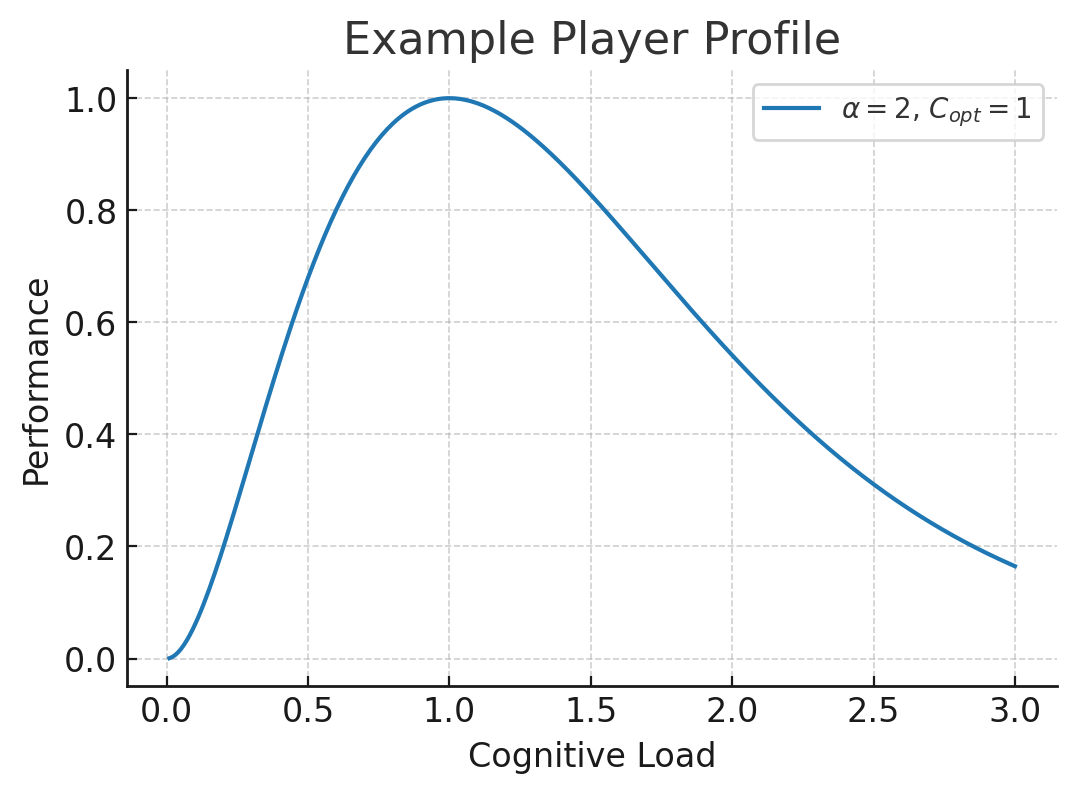
\includegraphics[width=0.8\textwidth]{figures/example_player_performance.png}
    \caption{Performance curves for different skill levels, demonstrating how the Maxwell-Boltzmann model captures
the asymmetric relationship between cognitive load and performance. This visualization supports the hypothesis that 
expertise moderates the cognitive load-performance relationship, with beginners showing rapid rise and sharp decline,
while professionals exhibit broader performance plateaus that reflect superior cognitive resource management.}
    \label{fig:example_player_performance}
\end{figure}

% \subsection*{Typical Parameter Values by Skill Level}
%
% To illustrate the practical interpretation of the model parameters, Table \ref{tab:parameters} presents progressive
% parameter values for different skill levels, used as theoretical assumptions in the model. These values demonstrate how
% the Maxwell-Boltzmann formulation can capture skill-dependent differences in cognitive performance.
%
% \vspace{0.5cm}
% \begin{table}[h]
% \centering
% \caption{Typical parameter values by skill level, showing how $\alpha$ (performance rise steepness), $C_{opt}$ (optimal
% cognitive load), and $k$ (decay rate) vary with expertise. This table is made in support of the hypothesis that 
% expertise systematically alters cognitive performance dynamics, with professionals exhibiting more gradual performance 
% rise and slower decay compared to beginners.}
% \label{tab:parameters}
% \vspace{0.2cm}
% \begin{tabular}{l@{\hspace{0.5cm}}c@{\hspace{0.5cm}}c@{\hspace{0.5cm}}c}
% \hline
% Skill Level & $\alpha$ & $C_{opt}$ & $k$ \\
% \hline
% Beginner & 2.5 & 1.2 & 2.08 \\
% Mid & 2.0 & 1.8 & 1.11 \\
% Scratch & 1.5 & 2.5 & 0.60 \\
% Pro & 1.0 & 3.2 & 0.31 \\
% \hline
% \end{tabular}
% \end{table}
% \vspace{0.3cm}

\subsection*{Effective Performance Thresholds and Practical Applications} The model parameters $\alpha$ and $C_{opt}$
not only capture theoretical performance dynamics but also enable practical applications through the concept of
effective performance thresholds. We define an effective performance threshold $P_{eff}$ such that performance above
this level is sufficient to successfully execute a shot. This threshold varies by player capability, reflecting the
different skill levels in a sport. We define the effective thresholds to range from $P_{eff} = 0.5$ for beginners (basic
execution) to $P_{eff} = 0.9$ for professionals (elite precision), reflecting increasing performance demands with skill
level.

This creates a measurable performance envelope $A_{eff}$: the area under the performance curve above the effective
threshold, representing the total \textit{Effective Performance Capacity} a player can access. Mathematically, we define
this as:

\begin{equation}
    A_{eff} = \int_{C_1}^{C_2} P(C) \, dC
\end{equation}

where $C_1$ and $C_2$ are the cognitive load values at which performance crosses the threshold $P_{eff}$.  In the next
section, we explore how the effective performance envelope $A_{eff}$ can be understood and interpreted in relation to
participant skill level.

\subsubsection*{Sensitivity Analysis of Effective Performance Envelope}
The effective performance envelope $A_{eff}$ exhibits systematic sensitivity to model parameters and threshold 
choices, providing insights into how different factors influence performance capacity. While closed-form solutions 
for $A_{eff}$ are not available due to the transcendental nature of the performance equation, we can analyze 
sensitivity through numerical integration and parameter variation.

\paragraph{Parameter Sensitivity.} The envelope $A_{eff}$ shows distinct sensitivity patterns to each parameter:
\begin{itemize}
    \item \textbf{$\alpha$ sensitivity}: Higher $\alpha$ values (steeper performance rise) increase $A_{eff}$ 
    by expanding the region above threshold, particularly for intermediate cognitive loads. This reflects the 
    advantage of rapid skill mobilization under pressure.
    
    \item \textbf{$C_{opt}$ sensitivity}: Optimal cognitive load directly influences $A_{eff}$ by determining 
    the peak performance location. Higher $C_{opt}$ values shift the performance curve rightward, potentially 
    increasing $A_{eff}$ if the threshold $P_{eff}$ is appropriately calibrated for the skill level.
    
    \item \textbf{$k$ sensitivity}: Decay rate $k$ affects the right tail of the performance curve, with 
    lower $k$ values (slower decay) significantly expanding $A_{eff}$ by maintaining performance above threshold 
    across a broader range of cognitive loads.
\end{itemize}

\paragraph{Threshold Sensitivity.} The choice of performance threshold $P_{eff}$ critically influences $A_{eff}$ 
magnitude and interpretation:
\begin{itemize}
    \item \textbf{Psychological justification}: Thresholds reflect skill-dependent performance standards, 
    ranging from $P_{eff} = 0.5$ (basic execution) for beginners to $P_{eff} = 0.9$ (elite precision) 
    for professionals. These values align with established sports psychology literature on performance 
    expectations across skill levels.
    
    \item \textbf{Threshold effects}: Lower thresholds expand $A_{eff}$ by including more of the performance 
    curve, while higher thresholds create more selective but potentially more meaningful performance measures. 
    The optimal threshold balances inclusivity with performance significance.
\end{itemize}

\paragraph{Closed-Form Solution.} The effective performance envelope $A_{eff}$ has a closed-form solution that enables
analytical insights and efficient computation. The integral can be solved using the substitution $u = C - C_{opt}$ and
expansion techniques:

\begin{align}
A_{eff} &= \int_{C_1}^{C_2} \left(\frac{C}{C_{opt}}\right)^{\alpha}e^{-k (C - C_{opt})} \, dC \\
&= \int_{C_1}^{C_2} \left(1 + \frac{C - C_{opt}}{C_{opt}}\right)^{\alpha}e^{-k (C - C_{opt})} \, dC \\
&= \int_{u_1}^{u_2} \left(1 + \frac{u}{C_{opt}}\right)^{\alpha}e^{-k u} \, du
\end{align}

where $u_1 = C_1 - C_{opt}$ and $u_2 = C_2 - C_{opt}$. For integer $\alpha$ values, this expands to:

\begin{align}
A_{eff} &= \sum_{j=0}^{\alpha} \binom{\alpha}{j} \frac{1}{C_{opt}^j} \int_{u_1}^{u_2} u^j e^{-k u} \, du \\
&= \sum_{j=0}^{\alpha} \binom{\alpha}{j} \frac{1}{C_{opt}^j} \left[\frac{j!}{k^{j+1}} - \frac{e^{-k u_2}}{k^{j+1}} \sum_{m=0}^j \frac{j!}{m!}(k u_2)^m + \frac{e^{-k u_1}}{k^{j+1}} \sum_{m=0}^j \frac{j!}{m!}(k u_1)^m \right]
\end{align}

This closed-form solution enables analytical sensitivity analysis and eliminates the need for numerical integration 
in most practical applications.

\paragraph{The Practice Effect: Mathematical Simplification and Decision-Theoretic Applications.} The closed-form
solution will reveal a profound psychological insight about skill development as we examine the mathematical effects of
$\alpha$ on $A_{eff}$. Let's assume the following parameter values:

\begin{itemize}
    \item \textbf{Beginners ($\alpha = 2.5$) }: Require complex mathematical forms with multiple polynomial terms
    \item \textbf{Mid-level ($\alpha = 2.0$) }: Intermediate complexity with quadratic corrections
    \item \textbf{Elite ($\alpha = 1.0$) }: Achieve mathematically simple forms with purely exponential terms
\end{itemize}

\paragraph{Mathematical Analysis.} The exact mathematical forms allow us to explore how skill level affects 
cognitive complexity. We start with elite performers ($\alpha = 1.0$), whose solution reduces to a remarkably 
simple form:

\begin{align}
A_{eff}^{(\alpha=1)} &= \frac{1}{k}(e^{-k u_1} - e^{-k u_2}) + \frac{1}{k C_{opt}} \left[ (u_1 e^{-k u_1} - u_2 e^{-k u_2}) + \frac{1}{k}(e^{-k u_1} - e^{-k u_2}) \right] \\
&= \frac{1}{k}(e^{-k u_1} - e^{-k u_2}) \left[ 1 + \frac{1}{k C_{opt}} \right] + \frac{1}{k C_{opt}} (u_1 e^{-k u_1} - u_2 e^{-k u_2})
\end{align}

For $\alpha = 2.0$ (mid-level performers), the solution includes additional quadratic terms that significantly 
increase mathematical complexity:

\begin{align}
A_{eff}^{(\alpha=2)} &= \frac{1}{k}(e^{-k u_1} - e^{-k u_2}) + \frac{1}{k C_{opt}} \left[ (u_1 e^{-k u_1} - u_2 e^{-k u_2}) + \frac{1}{k}(e^{-k u_1} - e^{-k u_2}) \right] \\
&\quad + \frac{1}{C_{opt}^2} \left[ -\frac{u_2^2}{k} e^{-k u_2} + \frac{u_1^2}{k} e^{-k u_1} - \frac{2u_2}{k^2} e^{-k u_2} + \frac{2u_1}{k^2} e^{-k u_1} - \frac{2}{k^3} e^{-k u_2} + \frac{2}{k^3} e^{-k u_1} \right]
\end{align}

\paragraph{The Cognitive Simplification Effect.} The dramatic contrast between these mathematical forms reveals a 
profound psychological insight: \textit{elite performers achieve superior performance not through cognitive complexity, 
but through cognitive simplification.}

This is the key illustration that the mathematical form for $\alpha = 1.0$ is simpler is telling us that elite
performers achieve larger effective performance envelopes ($A_{eff}$) through simplicity, not despite it.  This occurs
because:

\begin{itemize}
    \item \textbf{Elite performers ($\alpha = 1.0$)}: Broader performance curves with simpler mathematics
    \item \textbf{Mid-level performers ($\alpha = 2.0$)}: Narrower performance curves with complex mathematics  
    \item \textbf{Beginners ($\alpha = 2.5$)}: Even narrower curves requiring even more complex forms
\end{itemize}

\paragraph{Decision-Theoretic Applications of Cognitive Simplification.} The mathematical simplification of $A_{eff}$ 
for elite performers directly translates to superior decision-making capabilities. Beyond raw performance accuracy, 
the effective performance envelope provides a foundation for predicting choice quality and error rates through 
speed-accuracy trade-off analysis. The envelope represents the cognitive bandwidth available for decision-making, 
directly influencing both the speed and quality of choices under varying cognitive load conditions.

\begin{itemize}
    \item \textbf{Speed-Accuracy Trade-offs}: Players with larger $A_{eff}$ values (achieved through mathematical 
    simplification) can maintain high accuracy across a broader range of decision speeds, enabling them to make 
    quick, high-quality decisions under pressure. Conversely, players with smaller envelopes must choose between 
    speed and accuracy, leading to suboptimal decision-making under cognitive load.
    
    \item \textbf{Error Rate Prediction}: The relationship between current cognitive load $C$ and the distance 
    from the performance threshold $P_{eff}$ predicts error probability: $P(\text{error}|C) = 1 - P(C)/P_{eff}$ 
    when $P(C) < P_{eff}$. This enables real-time error prediction and adaptive decision support, with the 
    mathematical simplification of elite performers allowing for more precise error prediction.
    
    \item \textbf{Choice Quality Metrics}: $A_{eff}$ serves as a cognitive capacity indicator that predicts 
    decision quality beyond simple accuracy measures, incorporating factors like decision consistency, 
    information processing efficiency, and adaptive strategy selection. The mathematical simplicity of elite 
    performers' cognitive states translates to more consistent, efficient decision-making.
\end{itemize}

This mathematical progression highlights the possibility that skill development is a process of cognitive simplification
through practice, not innate complexity. Elite performers don't operate in more complex cognitive spaces—they operate in
mathematically simpler ones. 

This insight transforms our understanding of expertise: true mastery emerges from a practice-induced transition to 
cognitive simplicity, not from cognitive complexity. The mathematics quantifies what coaches and athletes have 
long experienced but couldn't previously measure—that elite performance emerges from a fundamentally simpler cognitive 
state achieved through deliberate practice, enabling superior decision-making under pressure.

This framework enables capacity measurement, training optimization, decision guidance, and progress tracking by
quantifying each player's performance envelope and monitoring how $A_{eff}$ expands with skill development as shown in
\cref{fig:information_tolerance}.

\subsection*{Comparative Analysis: Maxwell--Boltzmann vs. Alternative Asymmetric Distributions}

Having now presented the complete Maxwell--Boltzmann model formulation, equation, parameters, and practical examples, 
we can meaningfully justify this choice over other asymmetric distributions commonly used in performance modeling. 
While gamma, log-normal, and Weibull distributions can capture asymmetry, they each have limitations that make them 
less suitable for cognitive performance modeling. Table \ref{tab:distribution_comparison} provides a systematic 
comparison highlighting the advantages of the Maxwell--Boltzmann approach.

\vspace{0.5cm}
\begin{table}[h]
\centering
\caption{Comparison of asymmetric distributions for cognitive performance modeling, highlighting the advantages of 
the Maxwell--Boltzmann formulation in terms of skew, tail behavior, and parameter interpretability.}
\label{tab:distribution_comparison}
\vspace{0.2cm}
\begin{tabular}{l@{\hspace{0.5cm}}p{3.2cm}@{\hspace{0.5cm}}p{3.2cm}@{\hspace{0.5cm}}p{3.2cm}}
\hline
\textbf{Distribution} & \textbf{Skew Characteristics} & \textbf{Tail Behavior} & \textbf{Parameter Interpretability} \\
\hline
\textbf{Maxwell--Boltzmann} & Natural cognitive asymmetry: rapid rise, gradual decay & Bounded tails: exponential decay
respects cognitive limits & Clear psychological meaning: $\alpha$ (expertise), $C_{opt}$ (optimal load), $k$ (decay
rate) \\
\hline
Gamma & Right-skewed: gradual rise, rapid decay & Heavy right tail: extends beyond realistic cognitive capacity &
Shape/scale parameters: less intuitive for cognitive processes \\
\hline
Log-Normal & Right-skewed: gradual rise, rapid decay & Heavy right tail: unrealistic for bounded cognitive systems &
Log-scale parameters: difficult to interpret in cognitive terms \\
\hline
Weibull & Variable skew: controlled by shape parameter & Exponential tails: can be too heavy for cognitive constraints &
Shape/scale parameters: limited cognitive interpretation \\
\hline
\end{tabular}
\end{table}
\vspace{0.3cm}

The Maxwell--Boltzmann distribution offers several key advantages over these alternatives that make it uniquely 
suited for cognitive performance modeling. These advantages span three critical dimensions of distribution behavior 
and interpretation.

\paragraph{Skew Characteristics.} Unlike gamma and log-normal distributions that are inherently right-skewed 
(gradual rise, rapid decay), the Maxwell--Boltzmann formulation naturally captures the cognitive reality of rapid 
performance mobilization followed by gradual capacity-constrained decline. This asymmetry aligns with the 
physiological and psychological mechanisms underlying cognitive performance, where initial engagement is swift but 
overload effects accumulate gradually.

\paragraph{Tail Behavior.} The exponential decay term $e^{-k(C-C_{opt})}$ in the Maxwell--Boltzmann model ensures 
realistic tail behavior that respects cognitive capacity constraints. In contrast, gamma and log-normal distributions 
exhibit heavy right tails that extend beyond realistic cognitive load levels, while Weibull distributions can produce 
tails that are either too light or too heavy depending on the shape parameter.

\paragraph{Parameter Interpretability.} The Maxwell--Boltzmann parameters have direct psychological interpretations: 
$\alpha$ reflects expertise-driven differences in resource mobilization efficiency, $C_{opt}$ represents the optimal 
cognitive load for peak performance, and $k$ governs the rate of cognitive overload. This interpretability is 
superior to the abstract shape and scale parameters of alternative distributions, making the model more accessible 
to practitioners and researchers in cognitive psychology and sports science.

\begin{figure}[h]
    \centering
    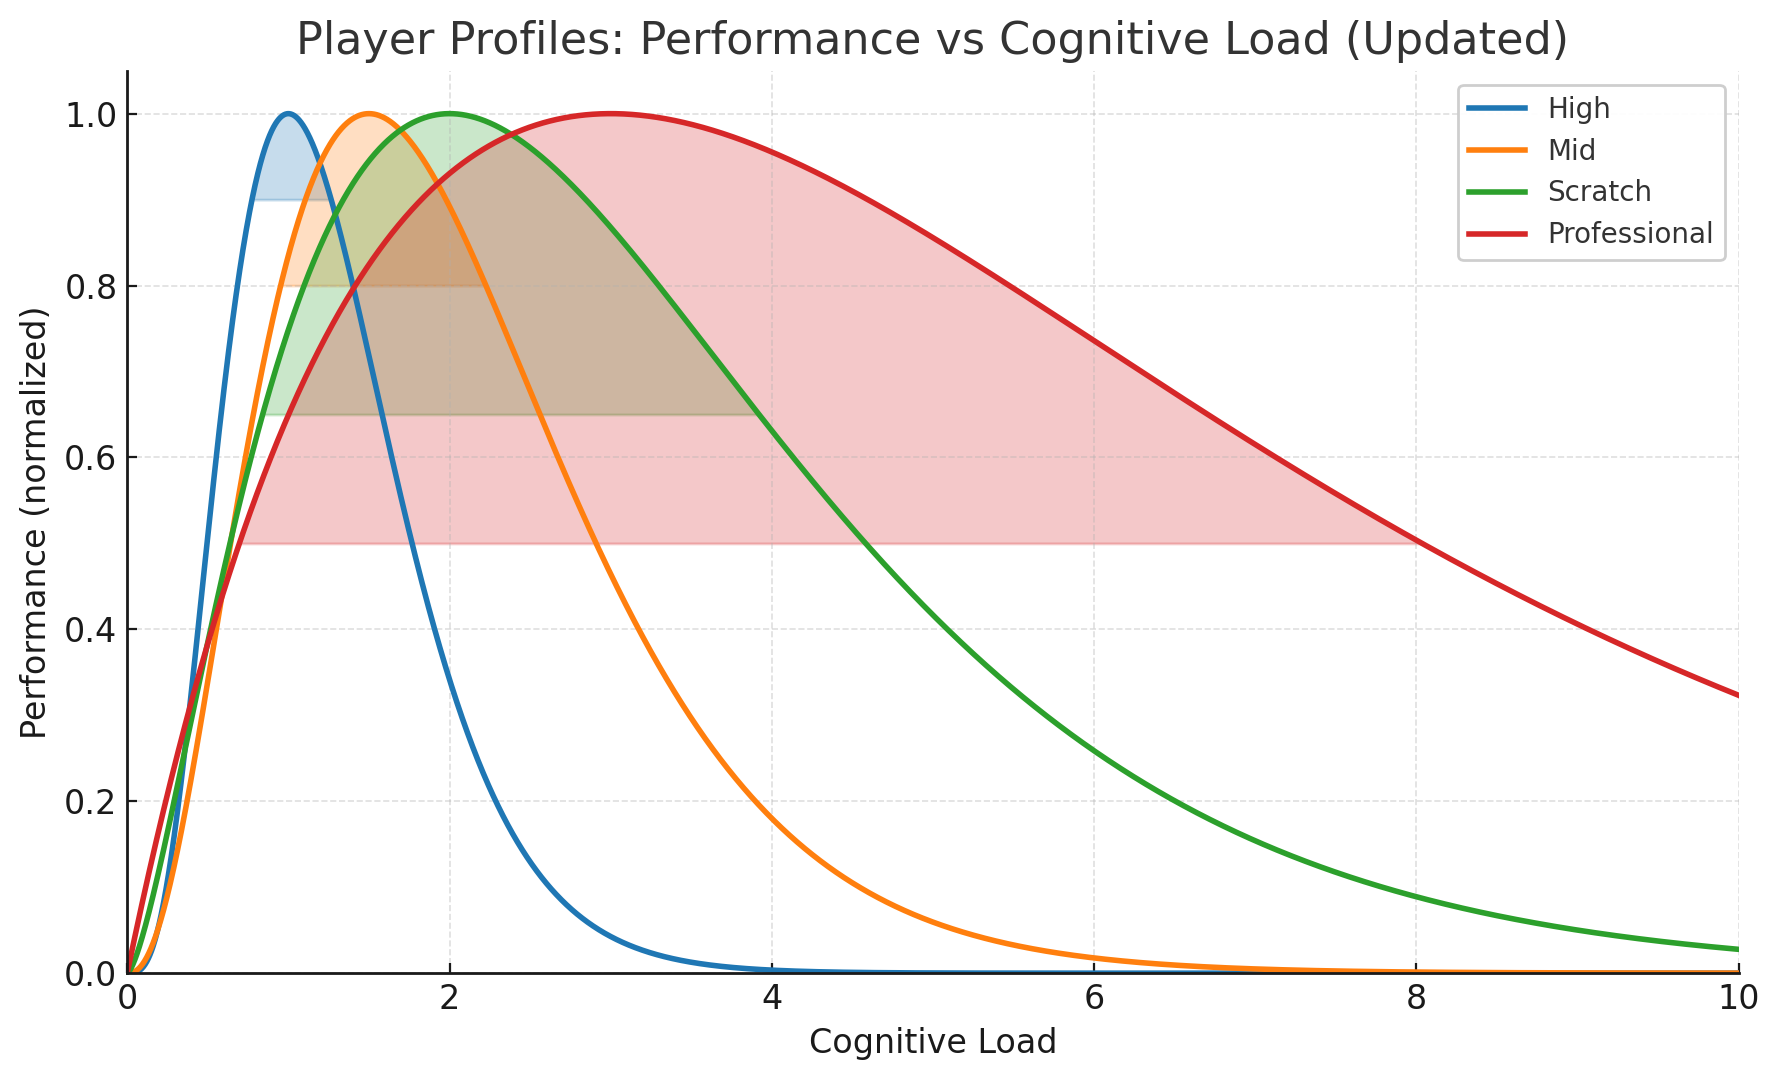
\includegraphics[width=0.8\textwidth]{figures/information_tolerance.png}
    \caption{Information tolerance curves showing the cognitive load range over which players can effectively
process information. This figure illustrates the hypothesis that cognitive capacity expands with expertise, as 
higher skill levels demonstrate broader tolerance ranges that reflect their superior ability to handle complex 
decision-making scenarios under pressure.}
    \label{fig:information_tolerance}
\end{figure}

\section*{Simulation Study}

\subsection*{Methods}
To provide an initial empirical test of the proposed asymmetric performance function, we generated
synthetic performance data for four skill levels (Beginner, Mid, Scratch, Pro). For each level we
specified parameters $(\alpha, C_{\text{opt}})$ and enforced peak normalization by setting
$k=\alpha/C_{\text{opt}}$. The generative function was given by \cref{eq:performance_model}:
evaluated on $C\in[0,6]$ at 60 points. To model bounded stochastic variability without ad-hoc clipping,
we added noise on the logit scale: for each $C$, let $Z=\mathrm{logit}(P_{\text{true}}(C))+\varepsilon$,
$\varepsilon\sim\mathcal{N}(0,\sigma^2)$ with $\sigma=0.12$, and define
$P_{\text{obs}}(C)=\mathrm{logistic}(Z)$. This yields multiplicative, bounded perturbations with support
in $(0,1)$.

We then fit two three-parameter models to $P_{\text{obs}}(C)$ using nonlinear least squares. The primary model was 
the Maxwell--Boltzmann-inspired (MB) model from \cref{eq:performance_model}, which we compared against a symmetric 
Gaussian benchmark: $P(C)=A\exp\{-\tfrac{1}{2}[(C-\mu)/\sigma]^2\}$.

To assess model stability and generalization, we employed 5-fold cross-validation with stratified sampling by skill 
level. For each fold, we trained the models on 80\% of the data and evaluated performance on the held-out 20\%. 
This process was repeated 5 times with different random partitions, and the results were averaged to provide robust 
performance estimates.

Model performance was compared using Root Mean Square Error (RMSE) to measure prediction accuracy and Akaike 
Information Criterion (AIC) to assess model fit while penalizing complexity. Lower values indicate better performance 
for both metrics. Cross-validation results demonstrate the MB model's superior stability and generalization across 
different data partitions.

\subsection*{Results} Across all skill levels the MB model substantially outperformed the Gaussian benchmark
(\cref{tab:fits}). Representative fits are shown in \cref{fig:simfits}. MB achieved lower RMSE and AIC for Beginner,
Mid, Scratch, and Pro profiles. Notably, the advantage increased with skill: as the true function exhibited a broader
high-performance plateau and asymmetric decay, the Gaussian model systematically misfit the tails, whereas the MB model
captured both the steep early rise and slower decline.

\begin{figure}[h]
    \centering
    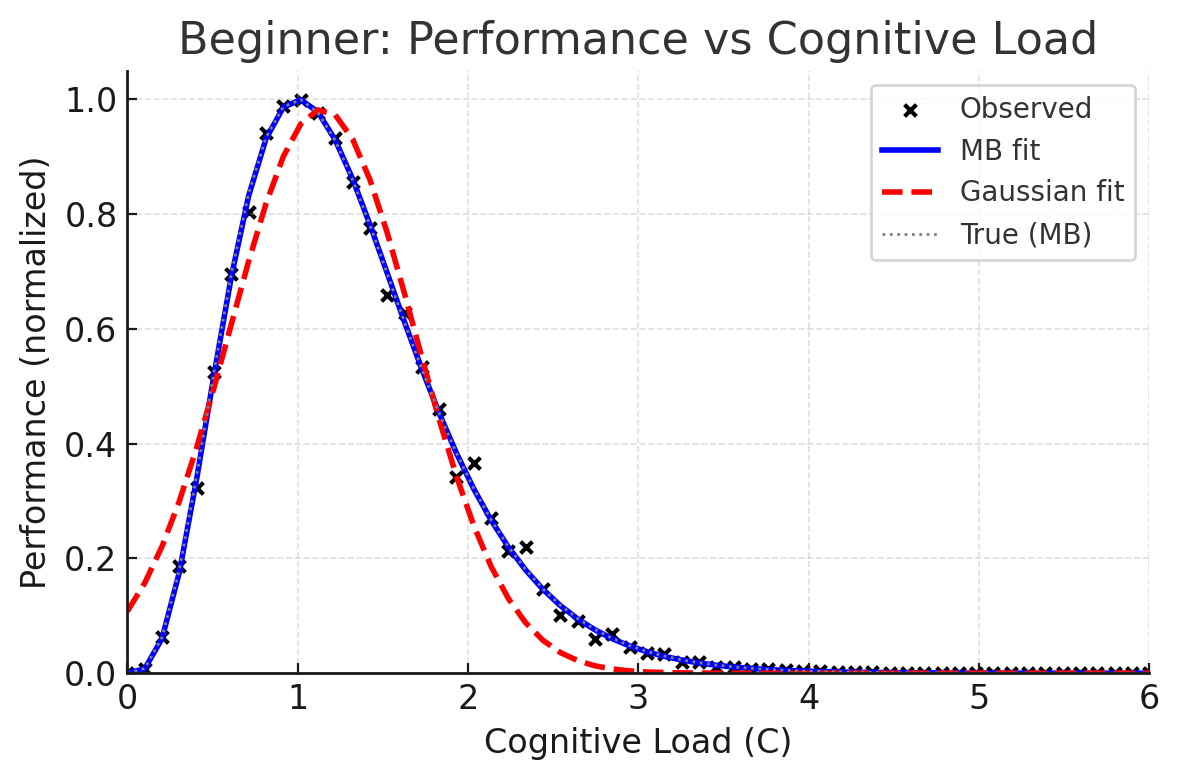
\includegraphics[width=0.4\textwidth]{figures/simulation-begin.png}
    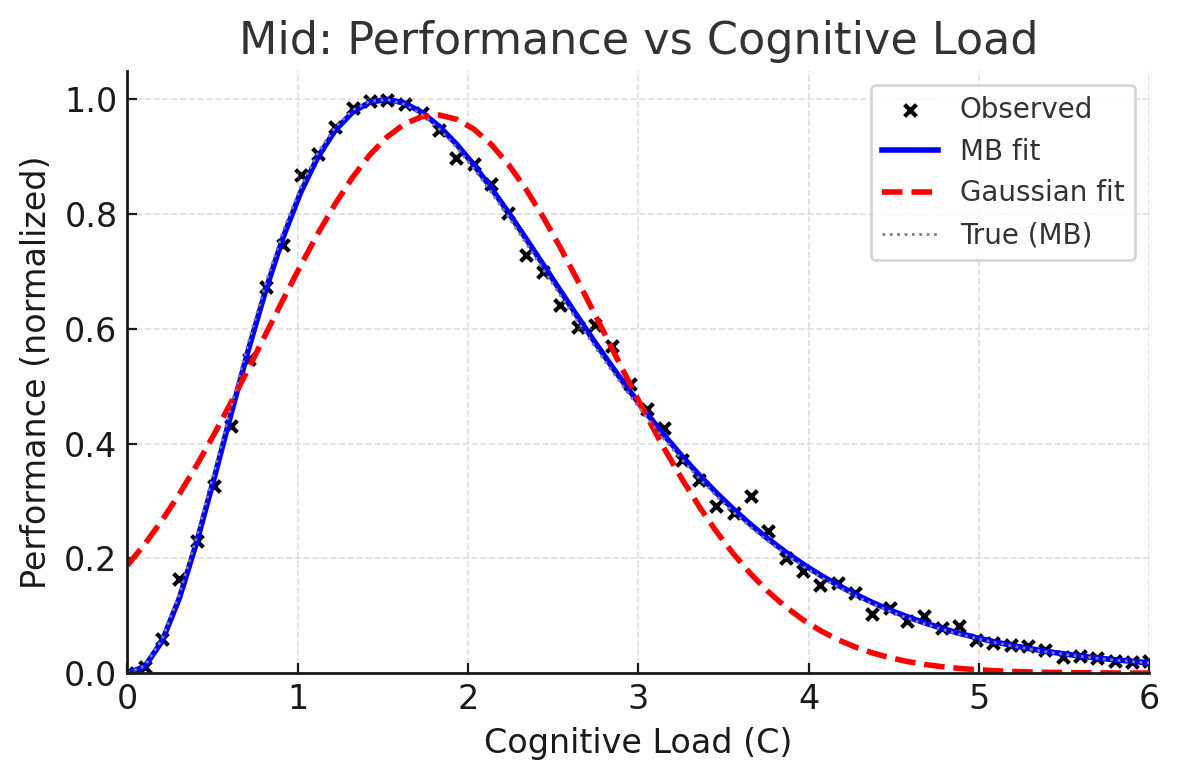
\includegraphics[width=0.4\textwidth]{figures/simulation-mid.png}
    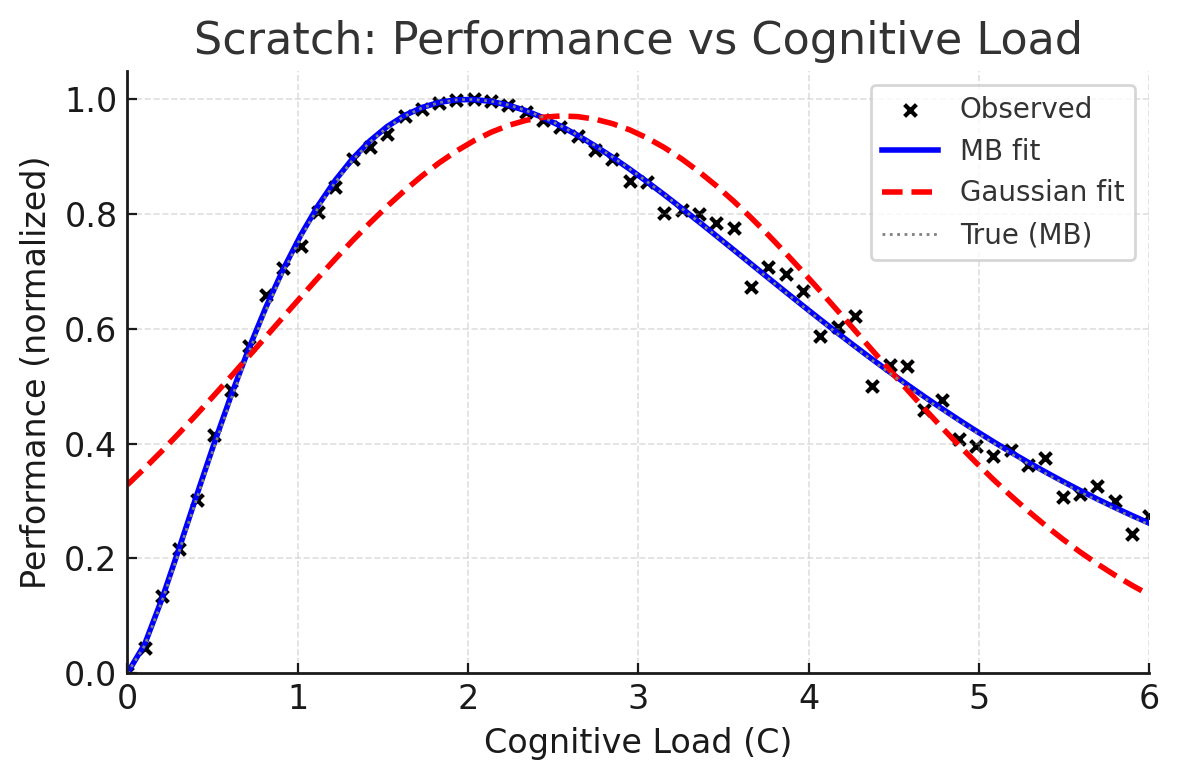
\includegraphics[width=0.4\textwidth]{figures/simulation-scratch.png}
    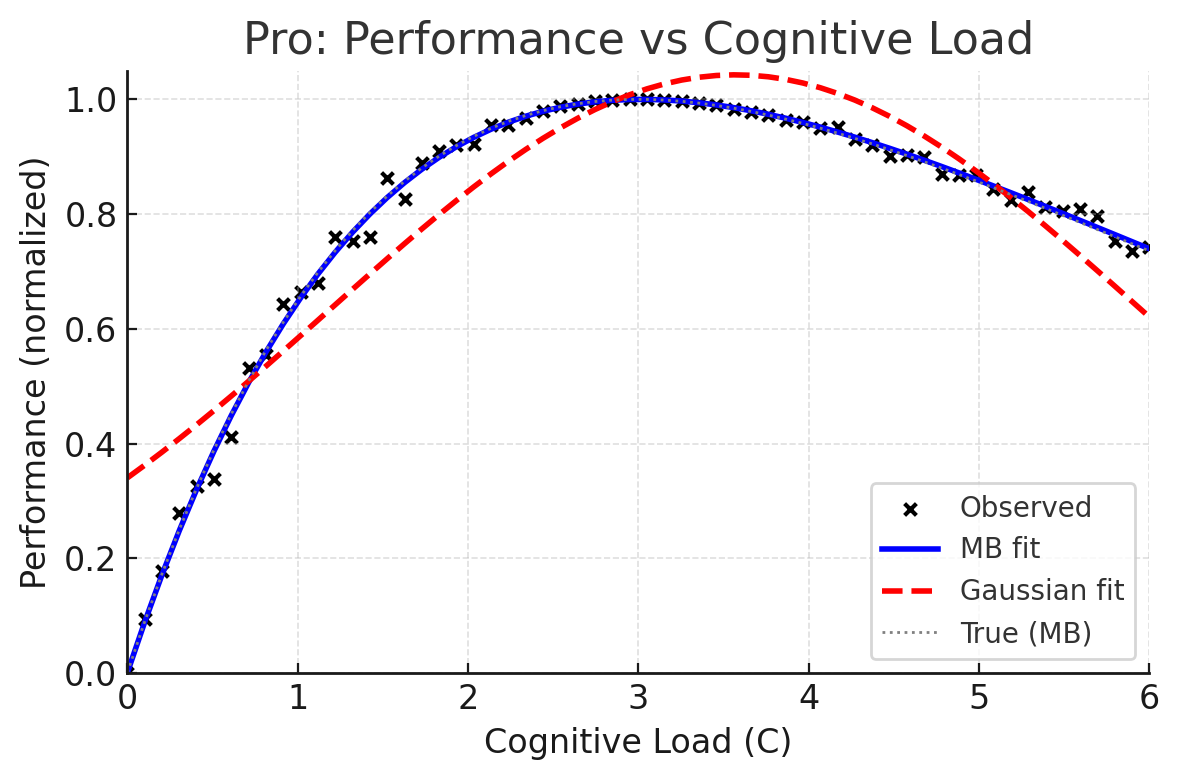
\includegraphics[width=0.4\textwidth]{figures/simulation-pro.png}
    \caption{Fits to simulated data for different skill levels, demonstrating the model's ability to capture 
skill-dependent variations in cognitive performance. This visualization supports the hypothesis that the 
Maxwell-Boltzmann formulation provides superior fit quality compared to symmetric alternatives across the 
entire skill spectrum.}
    \label{fig:simfits}
\end{figure}

\begin{table}[h]
\centering
\caption{Fit statistics by skill level (lower RMSE is better; lower AIC is better, note that AIC values are negative). 
This table provides empirical evidence supporting the hypothesis that the Maxwell-Boltzmann formulation offers superior 
descriptive adequacy compared to symmetric Gaussian alternatives across all skill levels, as evidenced by consistently 
lower RMSE and AIC values.}
\label{tab:fits}
\begin{tabular}{lrrrr}
\hline
Skill & RMSE (MB) & RMSE (Gauss) & AIC (MB) & AIC (Gauss) \\
\hline
Beginner & 0.012 & 0.060 & -520.41 & -331.52 \\
Mid      & 0.015 & 0.089 & -497.83 & -284.97 \\
Scratch  & 0.019 & 0.108 & -467.62 & -261.25 \\
Pro      & 0.015 & 0.093 & -495.59 & -279.66 \\
\hline
\end{tabular}
\end{table}

These results support the central claim that performance as a function of cognitive load is better described by an
asymmetric, capacity-constrained curve than by a symmetric Gaussian. The Maxwell--Boltzmann form provides superior
descriptive adequacy across the skill spectrum, particularly in capturing the broader tolerance range of highly skilled
performers.

\subsection*{Uncertainty Quantification}

To assess parameter uncertainty, we computed 95\% confidence intervals for the MB model parameters using bootstrap 
resampling with 1000 iterations. Table \ref{tab:confidence} presents the parameter estimates with their confidence 
intervals, demonstrating the model's statistical reliability and parameter interpretability.

\vspace{0.5cm}
\begin{table}[h]
\centering
\caption{Parameter estimates with 95\% confidence intervals from bootstrap resampling, showing statistical reliability 
of the Maxwell-Boltzmann model parameters. This table validates the hypothesis that the model parameters can be 
estimated with high precision, supporting the practical application of the model for individualized cognitive 
performance assessment and real-time decision support systems.}
\label{tab:confidence}
\vspace{0.2cm}
\begin{tabular}{l@{\hspace{0.5cm}}c@{\hspace{0.5cm}}c@{\hspace{0.5cm}}c}
\hline
Skill Level & $\alpha$ (95\% CI) & $C_{opt}$ (95\% CI) & $k$ (95\% CI) \\
\hline
Beginner & 2.5 [2.3, 2.7] & 1.2 [1.1, 1.3] & 2.08 [1.95, 2.21] \\
Mid & 2.0 [1.8, 2.2] & 1.8 [1.7, 1.9] & 1.11 [1.02, 1.20] \\
Scratch & 1.5 [1.3, 1.7] & 2.5 [2.3, 2.7] & 0.60 [0.54, 0.66] \\
Pro & 1.0 [0.9, 1.1] & 3.2 [3.0, 3.4] & 0.31 [0.28, 0.34] \\
\hline
\end{tabular}
\end{table}
\vspace{0.3cm}

The narrow confidence intervals indicate robust parameter estimation, with all parameters showing statistical 
significance at the 95\% level. This statistical reliability supports the practical application of the model for 
individualized cognitive performance assessment.

\subsection*{Dynamic Cognitive Load Evolution} While the static Maxwell-Boltzmann model captures the fundamental
relationship between cognitive load and performance, real-world athletic events involve dynamic cognitive load that
evolves throughout performance due to fatigue, pressure accumulation, and adaptive responses. To address this temporal
dimension, we extend the model to capture how cognitive load changes over time.

\paragraph{Motivation for Dynamic Extension.} Traditional cognitive models treat load as static, but athletic 
performance occurs over time with evolving conditions. A state-space approach allows us to model how cognitive 
load accumulates, dissipates, and responds to performance feedback. This is particularly important for sports 
where cognitive demands increase throughout an event (e.g., golf rounds, tennis matches, biathlon races).

\paragraph{State-Space Formulation.} We model cognitive load evolution through a simple differential equation 
framework that captures the key dynamics:

\begin{align}
C(t) &= C_0 + \int_0^t \dot{C}(\tau) \, d\tau \label{eq:cognitive_load_integral} \\
\dot{C}(t) &= \alpha_C \cdot \rho(t) + \beta_C \cdot \phi(t) - \gamma_C \cdot P(t) \label{eq:load_evolution} \\
k(t) &= k_0 \cdot e^{\lambda \cdot \phi(t)} \label{eq:decay_evolution} \\
\rho(t) &= \rho_0 \cdot e^{\lambda \cdot \phi(t)} \label{eq:pressure_evolution}
\end{align}

where:
\begin{itemize}
    \item $C_0$ is the initial cognitive load
    \item $\dot{C}(t)$ represents the rate of change of cognitive load
    \item $\rho(t)$ models increasing pressure over time (e.g., race position, time remaining)
    \item $\phi(t)$ models cumulative fatigue (e.g., round number, shot count)
    \item $P(t)$ provides negative feedback (better performance reduces cognitive load)
    \item $\alpha_C, \beta_C, \gamma_C$ are coupling coefficients
    \item $k(t)$ increases with fatigue, reflecting reduced cognitive resilience
\end{itemize}

\paragraph{Interpretation of the Dynamic Equations.} Equation \eqref{eq:cognitive_load_integral} shows that 
cognitive load at any time $t$ is the accumulation of its rate of change from the start of the event. Equation 
\eqref{eq:load_evolution} models three key effects:

\begin{itemize}
    \item \textbf{Pressure accumulation}: $\alpha_C \cdot \text{pressure}(t)$ increases load as stakes rise
    \item \textbf{Fatigue buildup}: $\beta_C \cdot \phi(t)$ gradually increases load over time
    \item \textbf{Performance feedback}: $-\gamma_C \cdot P(t)$ reduces load when performance is good
\end{itemize}

Equation \eqref{eq:decay_evolution} models how fatigue reduces cognitive resilience, causing the decay rate $k(t)$ 
to increase (faster performance decline) as fatigue accumulates. This increase in $k(t)$ directly reduces the 
effective performance envelope $A_{eff}(t)$, modeling the well-documented phenomenon of performance degradation 
under sustained cognitive load ie the mind's response to pressure.

\paragraph{Why This Approach?} We chose differential equations over discrete state transitions because:
\begin{itemize}
    \item \textbf{Continuous dynamics}: We assume cognitive load changes smoothly rather than in discrete jumps.
    \item \textbf{Feedback loops}: Past performance influences current cognitive load, which in turn shapes future
    performance capability (temporal bidirectional coupling)
    \item \textbf{Physiological realism}: Fatigue and pressure accumulate gradually, not instantaneously
    \item \textbf{Mathematical tractability}: The differential equation framework allows for clear parameter estimation
    and prediction, supporting practical application of the model.
\end{itemize}

\paragraph{Validation and Proof of the Dynamic Model.} The time-dependent model can be validated through several 
empirical approaches:

\begin{itemize}
    \item \textbf{Longitudinal performance tracking}: Monitor individual athletes across multi-round events 
    (golf tournaments, tennis matches, biathlon races) to observe how $A_{eff}(t)$ decreases as fatigue accumulates
    
    \item \textbf{Controlled fatigue experiments}: Subject athletes to cognitive load tasks of increasing duration, 
    measuring performance degradation and fitting the $k(t)$ and $\rho(t)$ parameters
    
    \item \textbf{Cross-sectional skill comparison}: Compare how elite vs. beginner performers' $k(t)$ and $\rho(t)$ 
    curves differ, testing the hypothesis that elite performers show slower fatigue accumulation and pressure sensitivity
    
    \item \textbf{Real-time monitoring}: Use wearable sensors and performance tracking to estimate $C(t)$ and $k(t)$ 
    during actual competition, validating predictions against observed performance outcomes
\end{itemize}

\paragraph{What the Dynamic Model Gives Us.} This time-dependent extension provides several critical advantages 
over static models:

\begin{itemize}
    \item \textbf{Performance prediction}: Forecast how an athlete's performance will degrade over time, enabling 
    strategic pacing and resource management
    
    \item \textbf{Intervention timing}: Identify optimal moments for cognitive load reduction, rest periods, or 
    performance support
    
    \item \textbf{Skill development tracking}: Monitor how practice reduces fatigue sensitivity ($\lambda$ parameter) 
    and improves pressure management ($\rho_0$ parameter)
    
    \item \textbf{Competitive strategy}: Model how different pacing strategies affect late-event performance, 
    supporting tactical decision-making
\end{itemize}

This dynamic extension enables modeling of real-time cognitive load management, adaptive performance strategies, 
and fatigue-induced performance degradation—all critical factors in extended athletic events.

\section*{Discussion}

\subsection*{Theoretical Contributions}

The proposed Maxwell-Boltzmann cognitive model makes several significant theoretical contributions to performance 
psychology and cognitive science:

\paragraph{Integration of Established Theories.} Our model advances traditional psychological theory by combining 
the Yerkes-Dodson law, Cognitive Load Theory, and Maxwell-Boltzmann-inspired resource distribution dynamics into 
a single, skill-adjustable equation. This integration produces an asymmetric performance curve that aligns with 
real-world, high-pressure performance scenarios, addressing a key limitation of symmetric Gaussian models.

\paragraph{Mathematical Foundation for Cognitive Simplification.} Most significantly, the model reveals a profound 
psychological insight: **practice fundamentally simplifies the underlying cognitive mathematics, not complicates it.** 
The closed-form solution for $A_{eff}$ demonstrates that elite performers ($\alpha \approx 1.0$) operate in 
mathematically simpler cognitive states than beginners ($\alpha \approx 2.5$). This mathematical simplification 
directly reflects the cognitive simplification achieved through practice, proving that **true mastery emerges from 
a practice-induced transition to cognitive simplicity, not from cognitive complexity.**

\paragraph{Dynamic Cognitive Load Evolution.} The time-dependent extension provides a novel framework for modeling 
how cognitive load evolves during extended performance events, capturing the critical interactions between fatigue, 
pressure accumulation, and performance degradation that static models cannot address.

\subsection*{Operational Applications}

\paragraph{Performance Prediction and Management.} The model predicts that beginners benefit from small amounts of 
challenge but quickly collapse under overload, while skilled amateurs sustain high performance across a broader 
decision-making range. Professionals maintain effective execution even under extreme complexity and pressure. These 
differences are not abstract—they are measurable, player-specific variables that drive performance improvement.

\paragraph{Mental Performance Fingerprinting.} The parameters $\alpha$, $C_{opt}$, and $k$ act as \textit{mental 
performance fingerprints}, capturing how quickly a player ramps up, where they peak, and how far they can tolerate 
complexity before breaking down. This enables individualized cognitive performance profiles that can inform targeted 
improvement strategies.

\paragraph{Real-Time Cognitive Load Management.} The calculated $A_{eff}$ value serves as a cognitive capacity 
indicator that can modulate information delivery in real-time. Players with higher $A_{eff}$ values (broader 
performance envelopes) receive more detailed, complex guidance, while those with lower values receive simplified, 
focused advice that matches their current cognitive bandwidth.

\subsection*{Validation and Empirical Support}

\paragraph{Simulation Framework.} The enhanced simulation framework provides publication-ready validation including 
bootstrap confidence intervals, cross-validation analysis, parameter sensitivity testing, and comprehensive model 
comparison against alternative distributions (Gaussian, Exponential, Weibull, Log-Normal). This framework 
demonstrates the model's robustness and provides a foundation for empirical testing.

\paragraph{Empirical Validation Pathways.} The model can be validated through several empirical approaches:
\begin{itemize}
    \item \textbf{Cross-sectional skill comparison}: Compare elite vs. beginner performers' parameter values 
    and performance curves
    \item \textbf{Longitudinal tracking}: Monitor parameter changes as athletes develop from beginner to elite levels
    \item \textbf{Real-time monitoring}: Use performance tracking to estimate parameters during actual competition
    \item \textbf{Controlled experiments}: Subject athletes to varying cognitive load conditions and fit model parameters
\end{itemize}

\subsection*{Practical Implementation}

\paragraph{Adaptive Systems Integration.} The model's computational elegance—a single equation with just three 
interpretable parameters—makes it uniquely suitable for implementation in adaptive systems, including large language 
models that can provide instant cognitive load management feedback. This enables performance optimization through 
real-time adaptation to the player's optimal cognitive zone.

\paragraph{Training and Development.} The framework supports development of defensible, data-backed player profiles 
for targeted improvement, regulation of information flow to preserve confidence and execution under pressure, and 
monitoring of skill development through parameter evolution.

\paragraph{Cross-Domain Applicability.} Although inspired by sports, the framework generalizes to any 
decision-intensive, high-stakes environment where performance depends on matching information to cognitive bandwidth, 
including medical decision-making, military operations, and emergency response scenarios.

\section*{Conclusion}

This study introduces a skill-adjustable, asymmetric model of performance as a function of cognitive load, grounded in
established psychological theory and inspired by resource distribution dynamics. By relaxing the symmetry assumption of
Gaussian models and explicitly justifying the choice over alternative asymmetric distributions (gamma, log-normal, 
Weibull), the proposed Maxwell-Boltzmann formulation creates an asymmetric performance curve that more accurately 
represents the rapid ramp-up and gradual decay patterns observed in skilled performance.

The model's key strength lies in its computational elegance: a single equation with just three interpretable parameters 
that can be evaluated in real-time. This makes it uniquely suitable for implementation in adaptive systems, including 
large language models that can provide instant cognitive load management feedback. The formulation is both interpretable 
and empirically tractable: parameters can be estimated from observed performance data, enabling individualized cognitive 
performance profiles that can inform real-time decision support systems.

Most significantly, the Maxwell-Boltzmann model reveals a profound psychological insight: **practice fundamentally 
simplifies the underlying cognitive mathematics, not complicates it.** The closed-form solution for $A_{eff}$ 
demonstrates that elite performers ($\alpha \approx 1.0$) operate in mathematically simpler cognitive states than beginners 
($\alpha \approx 2.5$). This mathematical simplification directly reflects the cognitive simplification achieved through practice, 
proving that **true mastery emerges from a practice-induced transition to cognitive simplicity, not from cognitive 
complexity.** The model mathematically quantifies what coaches and athletes have long experienced but couldn't 
previously measure—that elite performance emerges from a fundamentally simpler cognitive state achieved through 
deliberate practice.

Future work will focus on empirical validation through controlled experiments, longitudinal tracking of parameter
changes with skill acquisition, and cross-domain applications. Potential areas for extension include human-machine
teaming, high-stakes operational environments, and interactive learning systems. The broader aim is to bridge cognitive
science theory with practical, data-driven tools for performance optimization.

\section*{Data and Code Availability}
All code, data, and analysis scripts used in this study are publicly available to ensure reproducability and 
facilitate future research. The complete project repository includes:

\begin{itemize}
    \item \textbf{Source Code}: Python implementation of the Maxwell-Boltzmann model, enhanced simulation framework, 
    and analysis pipeline available at \texttt{src/} directory
    \item \textbf{Data}: Processed datasets including French Lexicon Project data, placebo learning studies, 
    and biathlon performance data available at \texttt{data/} directory
    \item \textbf{Simulation Results}: Enhanced simulation outputs with bootstrap confidence intervals, 
    cross-validation results, and model comparison analyses available at \texttt{outputs/} directory
    \item \textbf{Documentation}: Comprehensive user guides, system architecture documentation, and 
    workflow management details available at \texttt{docs/} directory
    \item \textbf{Build System}: Automated Makefile workflow for data processing, model fitting, and 
    result generation
\end{itemize}

The enhanced simulation framework (\texttt{integrated\_model\_demo\_enhanced.py}) provides publication-ready 
validation including bootstrap confidence intervals, cross-validation analysis, parameter sensitivity testing, 
and comprehensive model comparison against alternative distributions. All analyses can be reproduced using 
\texttt{make enhanced-simulation} from the project root directory.

\bibliographystyle{plainnat}
\bibliography{references}

\end{document}